\documentclass[12pt, a4paper]{article}
\usepackage{ctex}
\usepackage{graphicx}
\usepackage{float}
\usepackage[super, square]{natbib}
\usepackage{booktabs}
\usepackage[margin = 1in]{geometry}
\usepackage{
  color,
  clrscode,
  amssymb,
  ntheorem,
  amsmath,
  listings,
  fontspec,
  xcolor,
  supertabular,
  multirow
}
\renewcommand\contentsname{Contents}
\renewcommand\refname{References}
\renewcommand\figurename{Fig.}
\definecolor{bgGray}{RGB}{36, 36, 36}
\usepackage[
  colorlinks,
  linkcolor=bgGray,
  anchorcolor=blue,
  citecolor=black
]{hyperref}
\newfontfamily\courier{Courier}

\theoremstyle{margin}
\theorembodyfont{\normalfont}

\newtheorem{theorem}{Theorem}
\newtheorem{definition}[theorem]{Definition}
\newtheorem{example}[theorem]{Example}

\newcommand{\st}{\text{s.t.}}
\newcommand{\mn}{\mathnormal}
\newcommand{\tbf}{\textbf}
\newcommand{\fl}{\mathnormal{fl}}
\newcommand{\f}{\mathnormal{f}}
\newcommand{\g}{\mathnormal{g}}
\newcommand{\R}{\mathbf{R}}
\newcommand{\Q}{\mathbf{Q}}
\newcommand{\JD}{\textbf{D}}
\newcommand{\rd}{\mathrm{d}}
\newcommand{\str}{^*}
\newcommand{\vep}{\varepsilon}
\newcommand{\lhs}{\text{L.H.S}}
\newcommand{\rhs}{\text{R.H.S}}
\newcommand{\con}{\text{Const}}
\newcommand{\oneton}{1,\,2,\,\dots,\,n}
\newcommand{\aoneton}{a_1a_2\dots a_n}
\newcommand{\xoneton}{x_1,\,x_2,\,\dots,\,x_n}

\title{Project Report of RISC-V CPU\\\begin{large}(Course Project of Computer Architecture)\end{large}}
\author{Zhou Fan (范舟)\\ACM Class, Shanghai Jiao Tong University}
\date{}

\begin{document}

\lstset{numbers=left,
  basicstyle=\scriptsize\courier,
  numberstyle=\tiny\courier\color{red!89!green!36!blue!36},
  language=C++,
  breaklines=true,
  keywordstyle=\color{blue!70},commentstyle=\color{red!50!green!50!blue!50},
  morekeywords={},
  stringstyle=\color{purple},
  frame=shadowbox,
  rulesepcolor=\color{red!20!green!20!blue!20}
}
\maketitle

\section{Introduction}

GitHub repository of my CPU project: \url{https://github.com/Evensgn/RISC-V-CPU}

This project is a RISC-V CPU with five-stage pipeline, implemented in Verilog HDL. 

\section{Design}

\subsection{Features}

Main features of this RISC-V CPU are briefly introduced in the table below.

\begin{table}[H]
\centering
\begin{tabular}{@{}ll@{}}
\toprule
\multicolumn{1}{c}{Feature} & \multicolumn{1}{c}{RISC-V CPU}                                                                        \\ \midrule
ISA                         & RISC-V (\href{https://github.com/Evensgn/RISC-V-CPU/blob/dev/doc/inst-supported.md}{RV32I subset}) \\
Pipelining                  & 5 stages                                                                                              \\
Data forwarding             & complete forwarding path                                                                              \\
Cache                       & N-way set associate I-cache and D-cache\footnotemark[1]                                 \\
UART module                 & passed simulation \footnotemark[2] \\
Security                    & perfect proof against Meltdown and Spectre attack \footnotemark[3] \\
 \bottomrule
\end{tabular}
\end{table}

\begin{enumerate}
	\item The cache is based on Zhekai Zhang's (张哲恺) code\cite{zzk}. 
	\item UART module has not passed test on FPGA yet for the limited time. I re-designed part of CPU code to avoid hidden danger on FPGA, and it may need some more debugging.
	\item Just kidding ;-) That's because the CPU is not with branch prediction or out-of-order execution.
\end{enumerate}

\subsection{Specification}

The CPU has a standard 5-stage pipeline with complete path data forwarding. Data produced by EX stage or MEM stage is passed to ID stage, which avoids most of RAW data hazard under ideal conditions (causes stall only if producer is a load instruction).

The picture below shows structure of the CPU design, each module is implemented in a single verilog file. Red paths show the stall control flow, while orange ones show data forwarding path.

\begin{figure}[H]
	\begin{center}
	  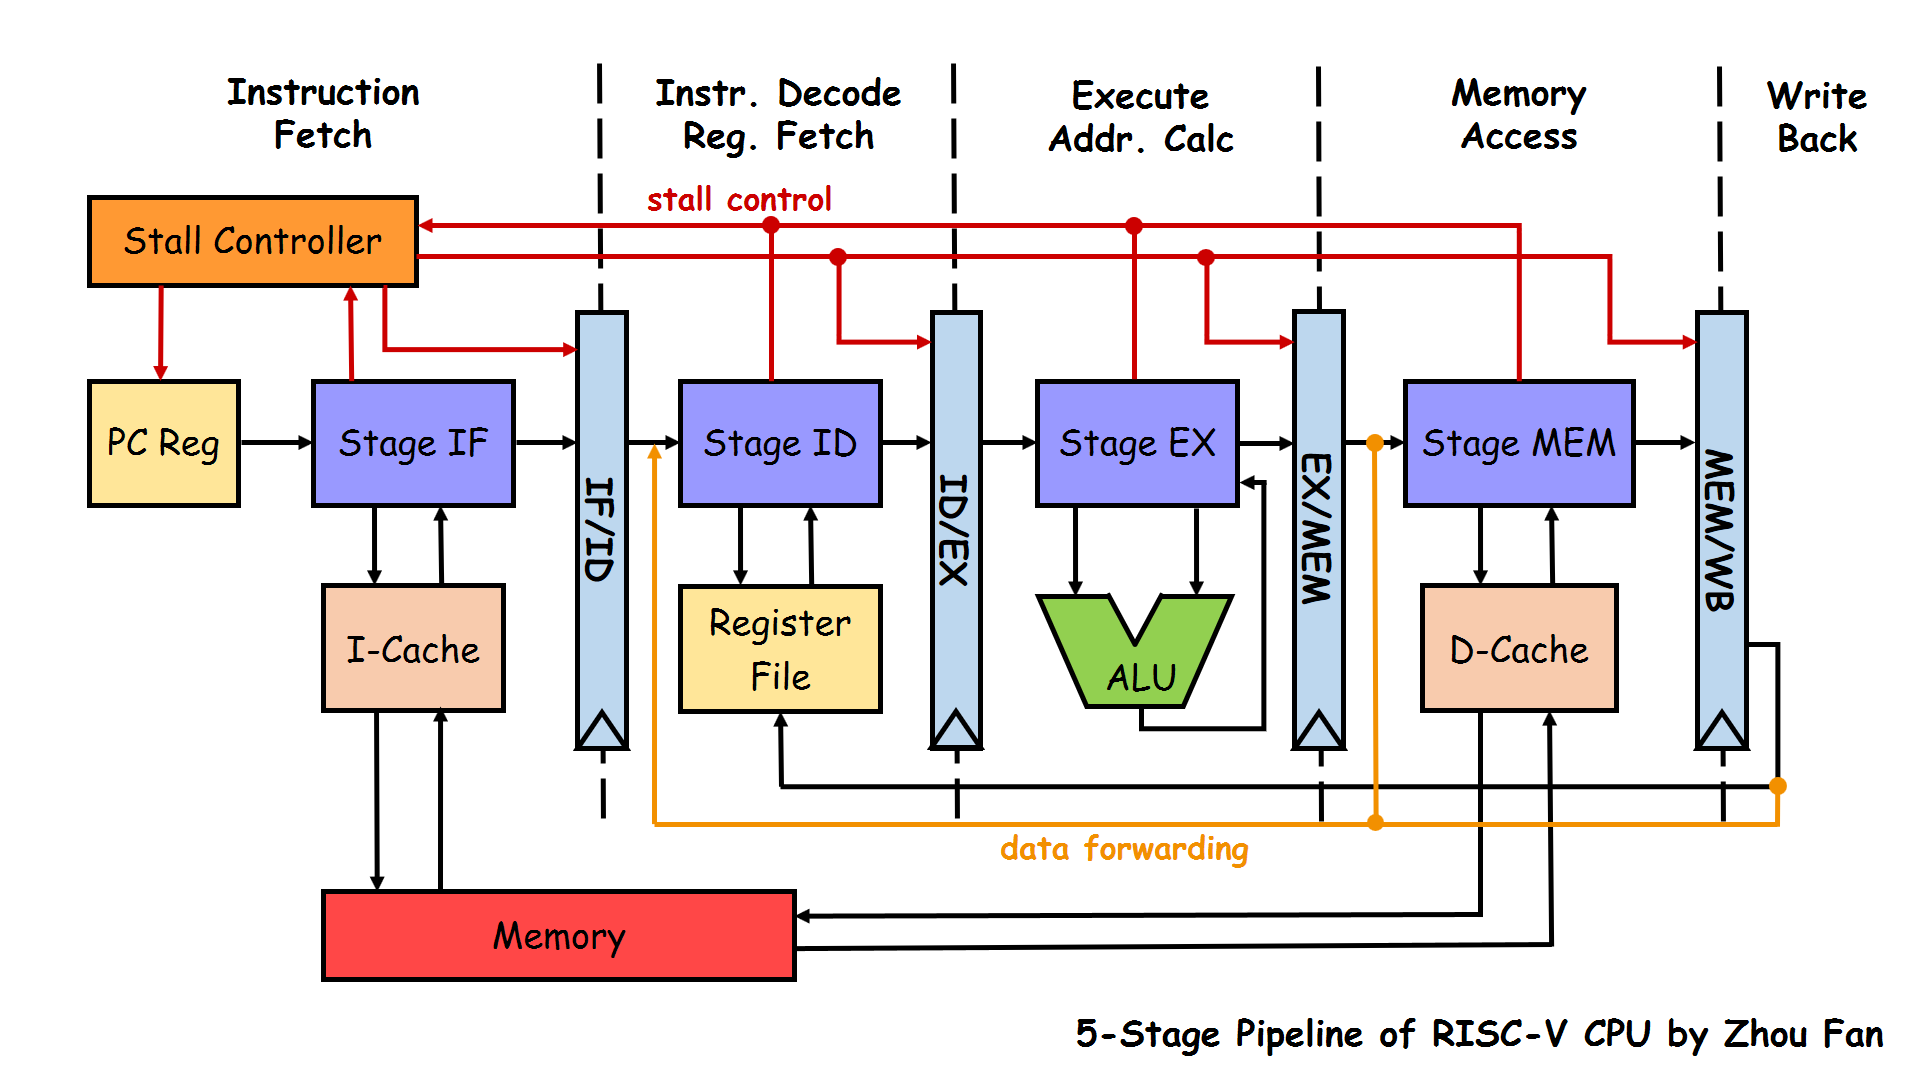
\includegraphics[height=9cm]{cpu-pipeline-graph.png}
	\end{center}
	\caption{Overview of CPU Design}
\end{figure}

\begin{itemize}
	\item Instruction fetching, Load/Store instruction or data dependency may cause stall of pipeline, the logic of stall is managed by a stall controller module. It receives stall requests from IF/ID/MEM stage, and emit stall signals to modules that should pause.

	\item For program test on FPGA without capable memory, the CPU uses UART protocol to communicate with PC, where runs a memory simulator written in C++.

	\item Latency of UART communication makes it significant to use a cache, the cache is N-way associate using LRU replacement policy. It is based on code from Zhekai Zhang's MIPS CPU project.
\end{itemize}

The CPU with cache and UART module passed simulation in Xilinx Vivado using multiple test programs. But something goes wrong when tested on FPGA (Basys 3), which is explained in the next section.

\begin{figure}[H]
	\begin{center}
	  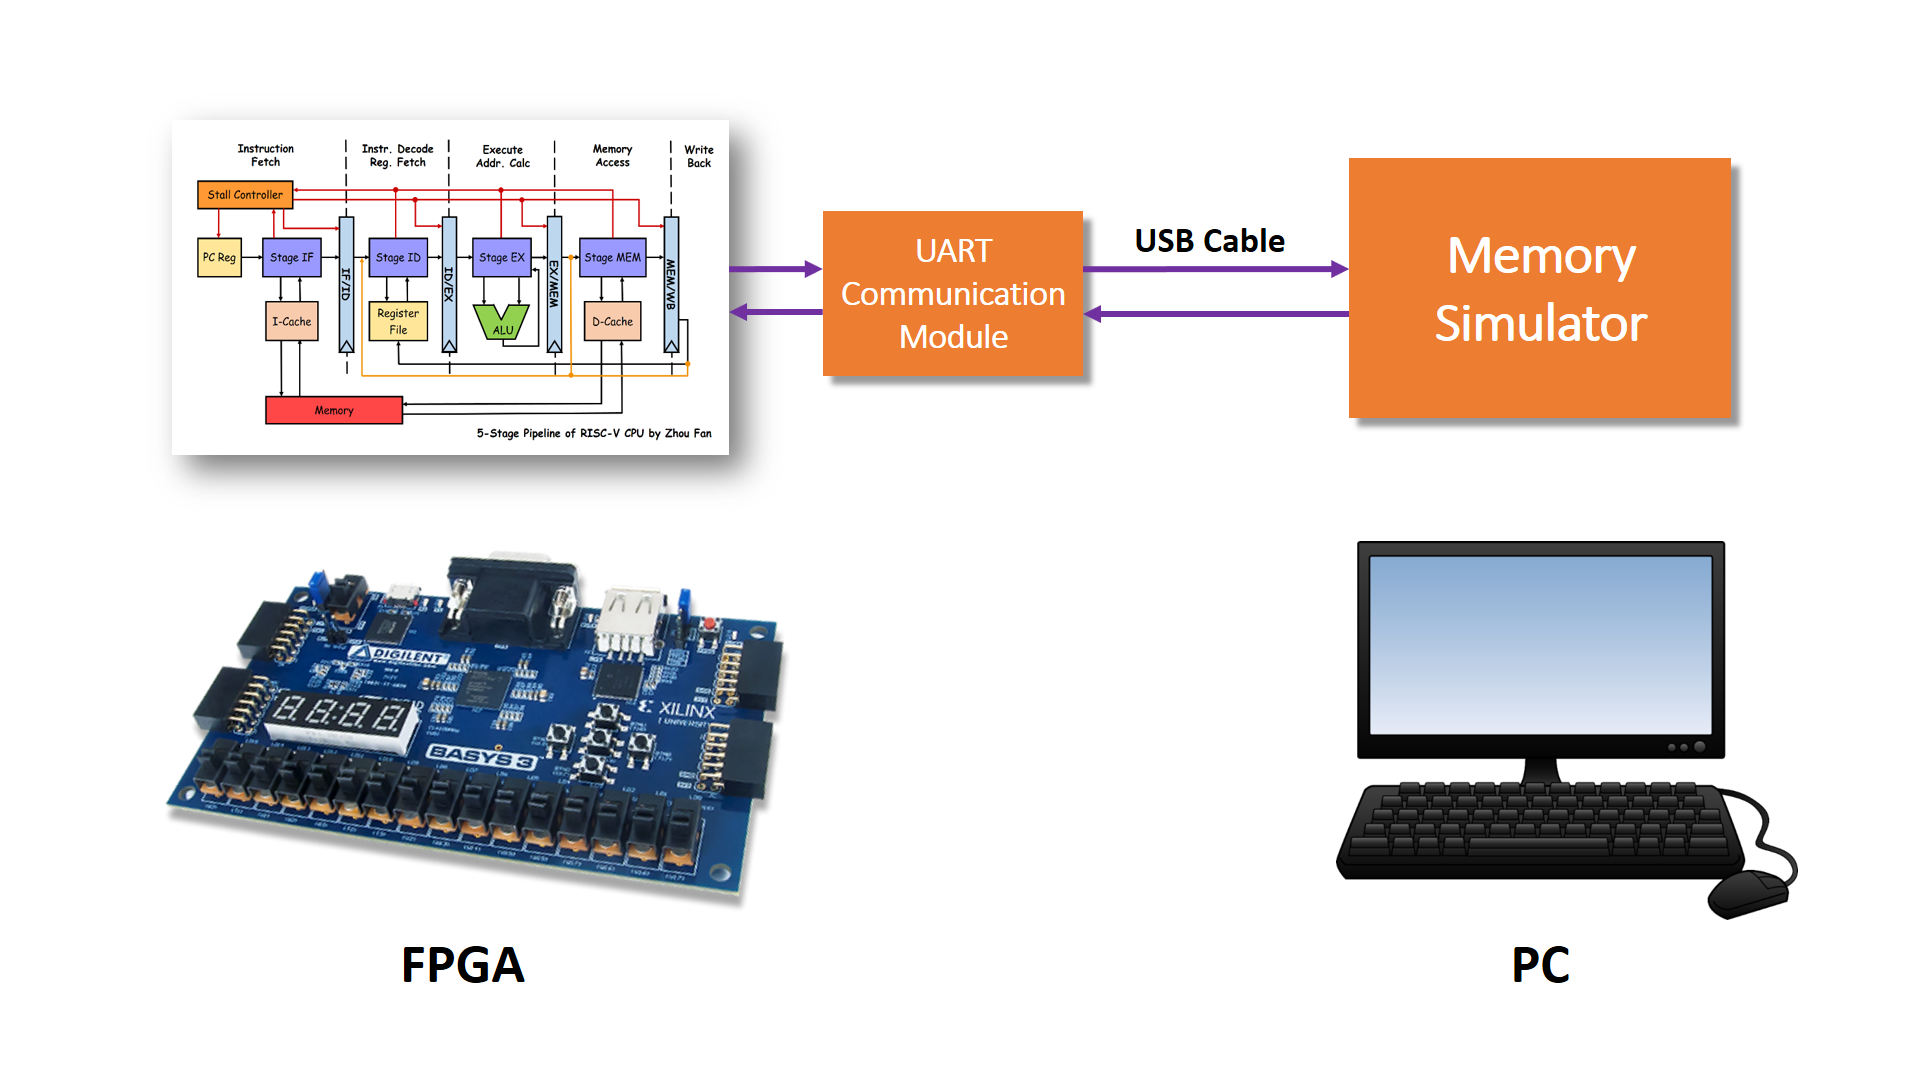
\includegraphics[height=9cm]{uart-simulate-memory.png}
	\end{center}
	\caption{Communication with memory simulator using UART protocol}
\end{figure}

\section{Thinkings}

\paragraph{Efficiency} Time efficiency is always a significant issue in CPU design. When I wrote code for stall logic and Branch/Jump instruction processing part, I tried to minimize number of unused clock cycle. But when UART latency is considered, all of those optimization lose their meaning: UART communication is the only bottleneck of the pipeline, and even the pipeline is not a pipeline any more, for an instruction would goes through all stages before the next instruction is fetched. Though there is I-cache, it only works for loops. Therefore, UART may not be a perfect solution to memory simulation.

\paragraph{Experience with FPGA} After cache and UART module passed simulation, I tested the CPU on Basys 3 FPGA, it read the first 5 instructions correctly but did not jump at the 5th instruction, which is a branch instruction. That test program did not go wrong in Vivado simulation. In the last two days before deadline I tried to find the bug but did not make it. Zhanghao Wu gave me a tutorial about always @ blocks\cite{always}, from which I learned about latch generation. My original design for stall control with IF stages caused some latch inferring, which could be "a
terrible place for bugs"\cite{always}. I re-designed part of code to avoid latches, and found that it may need some more debugging. From this experience, I learned that some hidden trouble would not reveal itself in simulation. And I should have learned more about Verilog HDL before starting to write code.

\paragraph{Automation} To compile and assemble test programs RISC-V toolchain and some other tools are used. Many commands are needed in this process. I \href{http://blog.evensgn.com/riscv-gnu-toolchain/}{wrote a Makefile} and found it really helpful. Automation improves efficiency and it feels good!

\section{Acknowledgements}
Special thanks would go to Zhanghao Wu (吴章昊) for his instructive discusstions and useful suggestions on this project. I would like to express my gratitude to TA Zhekai Zhang (张哲恺) as well, for his MIPS CPU project (especially the code of cache and UART module) and much work for this assignment. I am also indebted to many other classmates for their direct and indirect help to me.

\section{Appendix}

\begin{figure}[H]
	\begin{center}
	  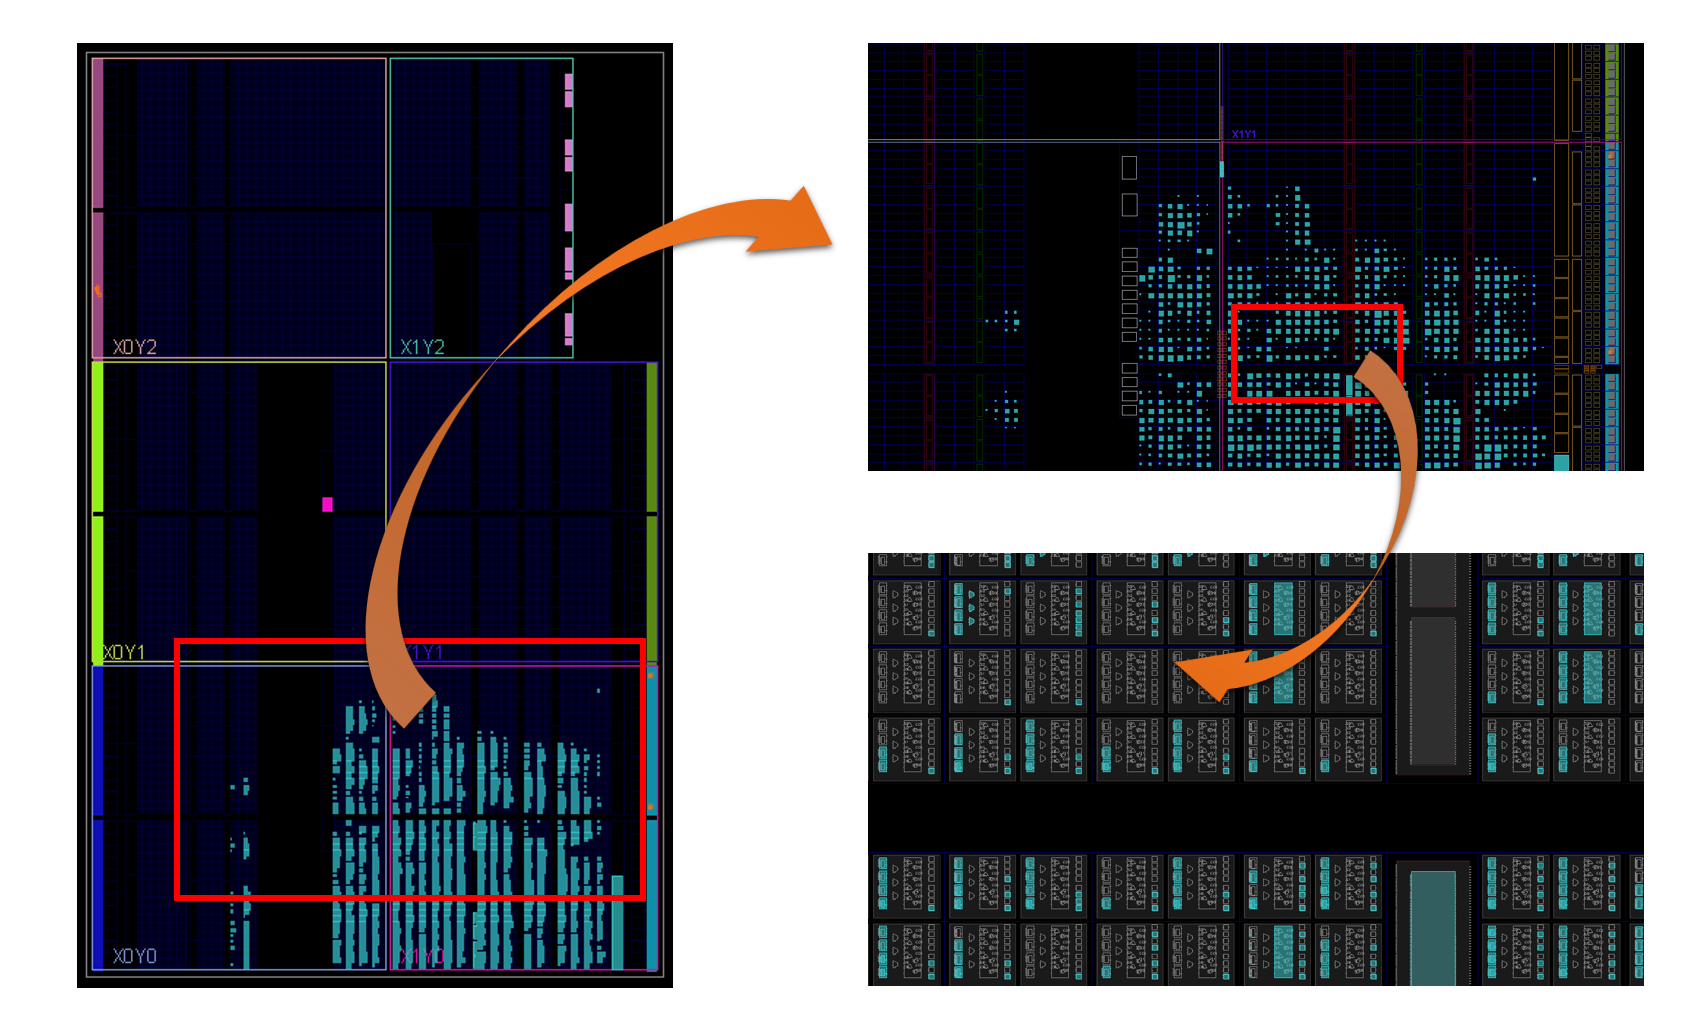
\includegraphics[height=9.5cm]{implementation-graph.png}
	\end{center}
	\caption{Implementation on Basys 3 FPGA, using Xilinx Vivado}
\end{figure}

\begin{figure}[H]
	\begin{center}
	  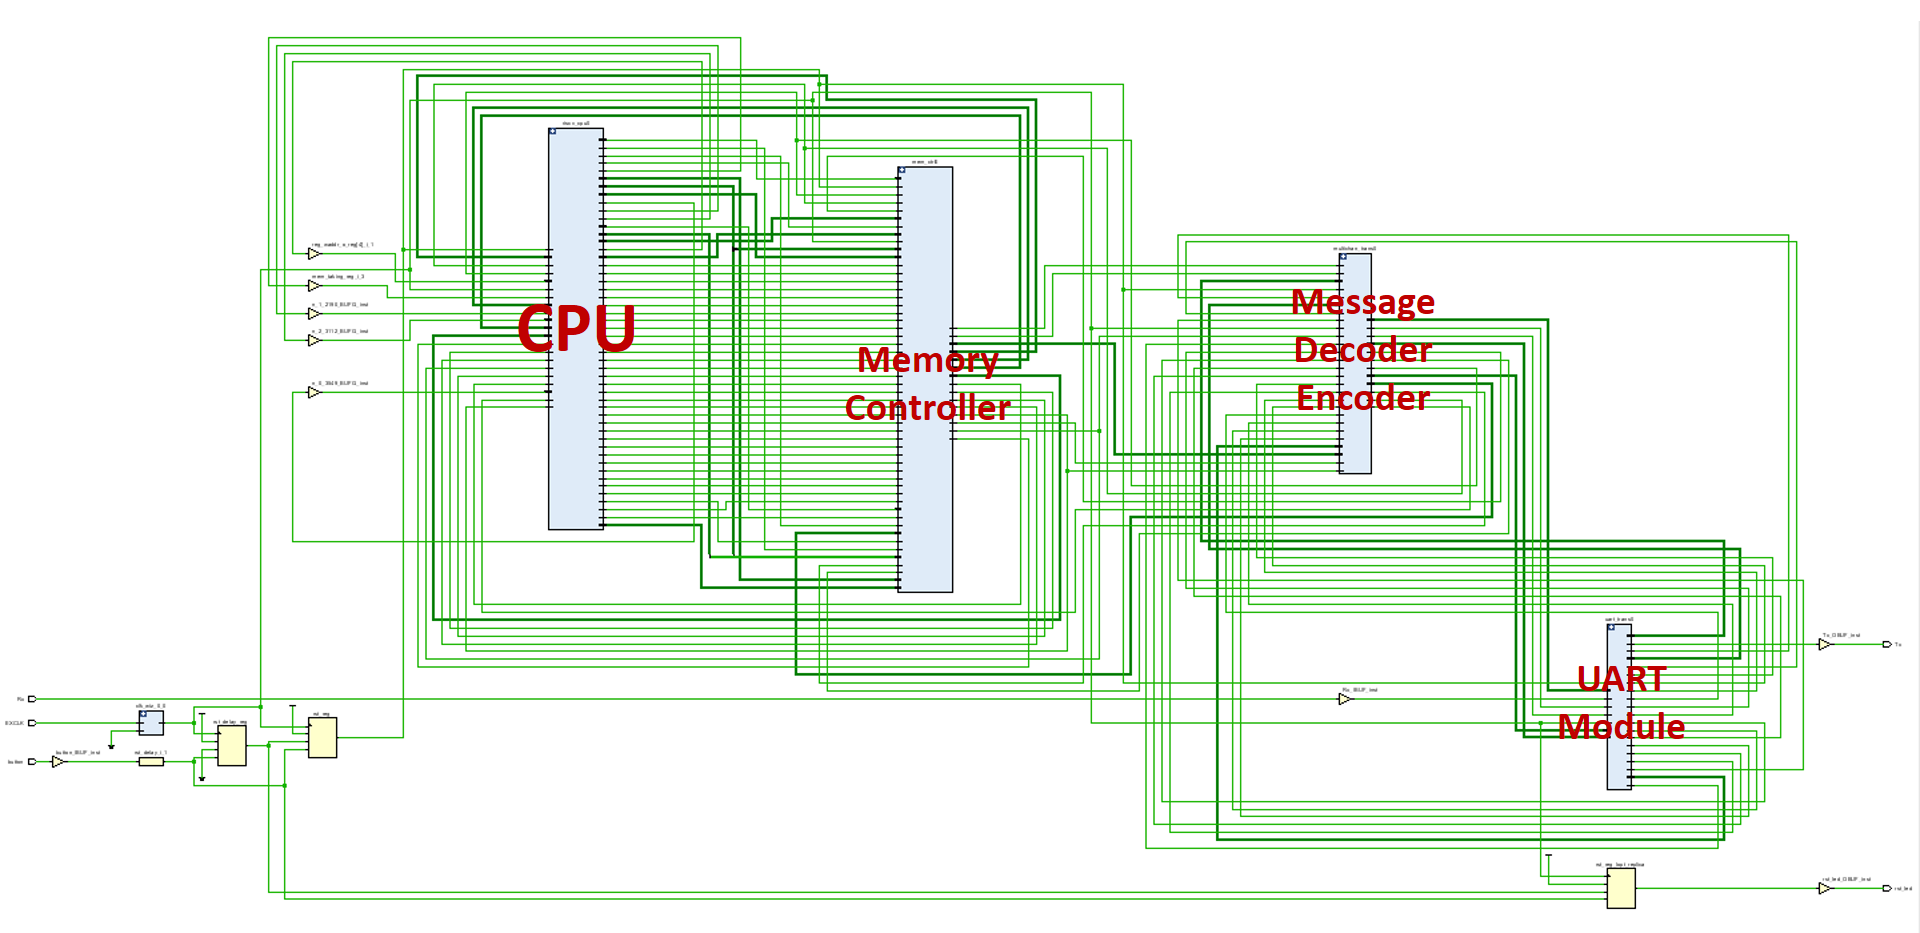
\includegraphics[height=8cm]{implementation-circuit-overview-captioned.png}
	\end{center}
	\caption{Scematic Overview}
\end{figure}

\begin{figure}[H]
	\begin{center}
	  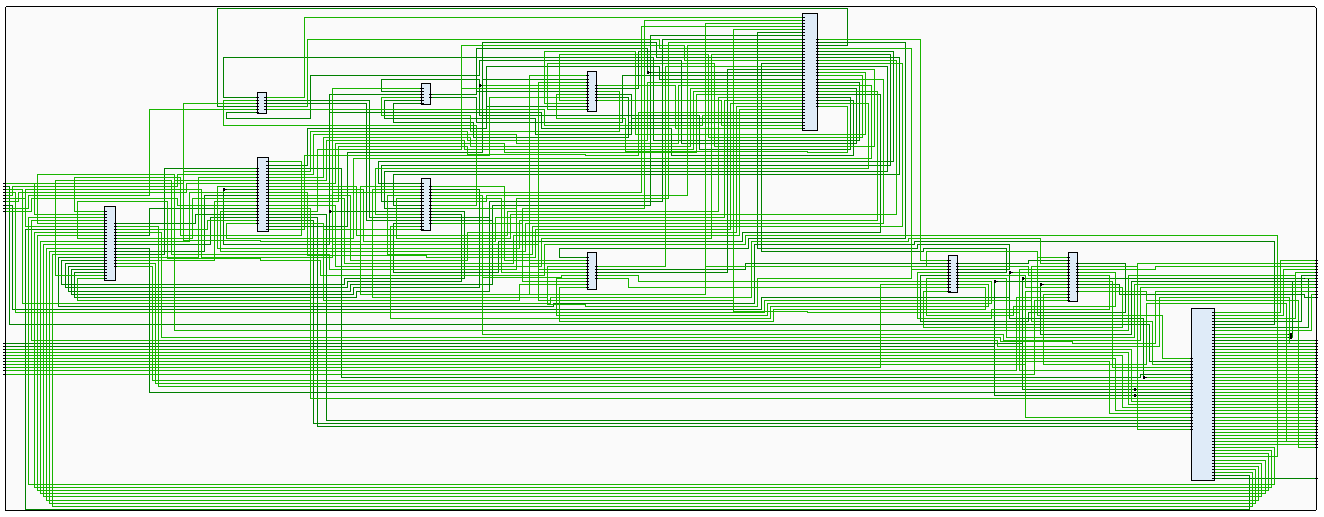
\includegraphics[height=6.5cm]{implementation-circuit-cpu.png}
	\end{center}
	\caption{CPU Module Scematic}
\end{figure}

\begin{thebibliography}{9}
  \bibitem{lsl}
  	雷思磊.
  	\emph{自己动手写CPU},
  	电子工业出版社, 2014.
  \bibitem{caqa} 
	John L. Hennessy, David A. Patterson, et al.
	\emph{Computer Architecture: A Quantitative Approach},
	Fifth Edition, 2012.
  \bibitem{ppt}
	David A. Patterson.
	PPT of \emph{CS252 Graduate Computer Architecture},
	2001.
  \bibitem{zzk}
  	Zhekai Zhang's (张哲恺) MIPS CPU project.
  	\url{https://github.com/sxtyzhangzk/mips-cpu}
  \bibitem{always}
  	Chris Fletcher.
  	\emph{\href{https://github.com/Evensgn/RISC-V-CPU/blob/dev/doc/Always@.pdf}{Verilog: always @ Blocks}}
  
\end{thebibliography}

\end{document}